\section{Hướng dẫn sử dụng các tính năng của chương trình}

\subsection{Yêu cầu}
Để sử dụng được chương trình, máy tính phải cài đặt Python 3 và các thư viện ở phần \ref{env}.

\subsection{Khởi động server}
Để khởi động server, ta vào đường dẫn chứa các tập tin mã nguồn của server, mở terminal và sử dụng câu lệnh: \lstinline[language=bash]{python main.py} hoặc \lstinline[language=bash]{python3 main.py}.
\begin{figure}[H]
\center{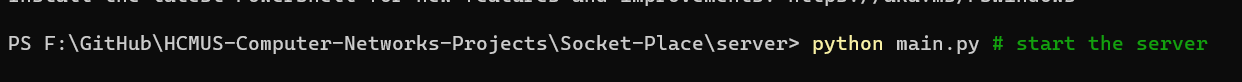
\includegraphics[scale=0.6]{instructions/start_server}}
\caption{Khởi động server}
\end{figure}

\subsection{Khởi động client}
Để khởi động client, ta vào đường dẫn chứa các tập tin mã nguồn của client, mở terminal và sử dụng câu lệnh: \lstinline[language=bash]{python main.py} hoặc \lstinline[language=bash]{python3 main.py}.
\begin{figure}[H]
\center{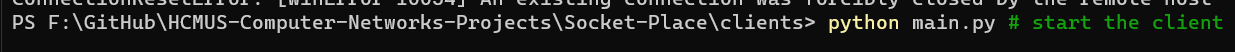
\includegraphics[scale=0.6]{instructions/start_client}}
\caption{Khởi động client}
\end{figure}

\subsection{Giao diện khởi động client}
Sau khi khởi động, client có giao diện như sau:
\begin{figure}[H]
\center{\includegraphics[scale=0.6]{instructions/client_first_gui}}
\caption{Khởi động client}
\end{figure}
Giao diện khởi đầu của client là danh sách các địa điểm đang được server quản lý, các thông tin hiển thị bao gồm: ID địa điểm và tên địa điểm.\\
Trên giao diện khởi đầu, nút \textbf{Xem chi tiết} bên cạnh tên mỗi địa điểm cho phép ta truy vấn thông tin chi tiết về địa điểm đó từ server; nút \textbf{Tải về hình ảnh} bên cạnh mỗi địa điểm cho phép ta tải về các hình ảnh của địa điểm đó từ server, hình ảnh sau khi tải về được lưu trong thư mục \textbf{\textit{Temp}} và được hiển thị lên GUI.\\
Ở phía dưới cùng của giao diện là nút \textbf{Tải tất cả hình ảnh đại diện}, cho phép ta tải về hình ảnh đại diện của tất cả các địa điểm đang được quản lý bởi server. Hình ảnh sau khi tải về được xử lý tương tự bên trên.

\subsection{Truy vấn thông tin chi tiết một địa điểm}
Nút \textbf{Xem chi tiết} ở giao diện khởi đầu cho phép client truy vấn thông tin chi tiết, được lưu tại server, về địa điểm tương ứng. Các thông tin hiển thị lên màn hình gồm: mã số địa điểm, tên địa điểm, tọa độ (vĩ độ, kinh độ) của địa điểm, mô tả và hình đại diện. Hình \ref{query1} là ví dụ về truy vấn thông tin chi tiết một địa điểm.
\begin{figure}[H]
\center{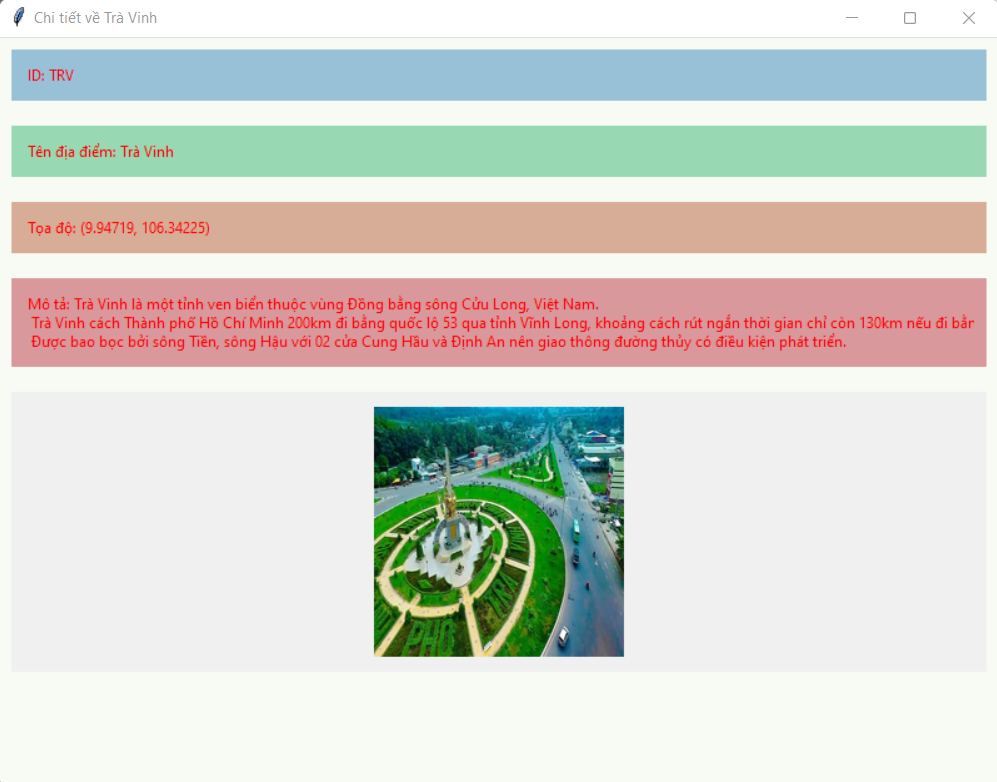
\includegraphics[scale=0.8]{instructions/query_one}}
\caption{Truy vấn thông tin chi tiết một địa điểm}
\label{query1}
\end{figure}

\subsection{Tải tất cả hình ảnh dại diện}
\label{down_all_avt}
Nút \textbf{Tải tất cả hình ảnh đại diện} cho phép client tải về tất cả hình ảnh đại diện của các địa điểm từ server. Hình ảnh sau khi tải về được lưu trong thư mục \textbf{\textit{Temp}} và được hiển thị lên giao diện của client. Các nút \textbf{Hình kế} và \textbf{Hình trước} tương ứng cho ta xem hình ảnh kế tiếp và hình ảnh ngay trước của hình ảnh hiện tại. Hình \ref{all1}, \ref{all2} và \ref{all3} là ví dụ về tải tất cả hình ảnh đại diện.
\begin{figure}[H]
\center{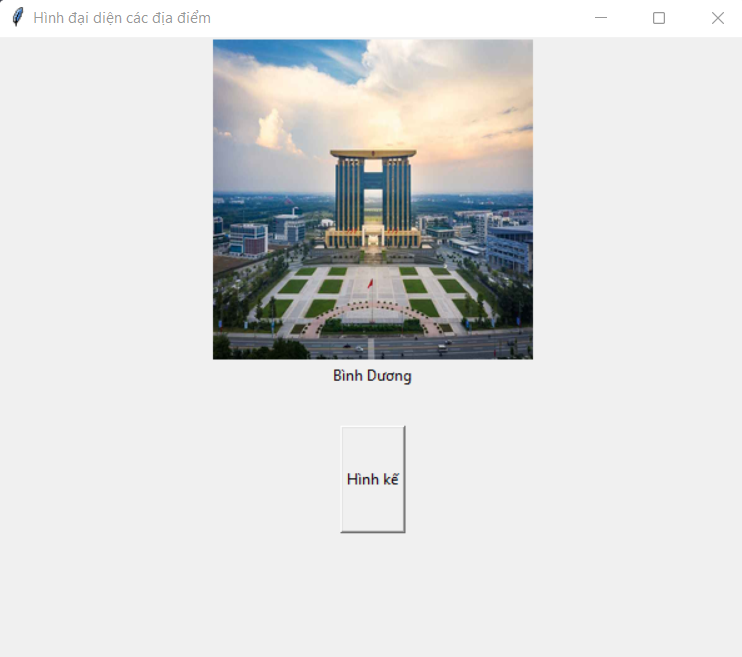
\includegraphics[scale=0.8]{instructions/down_all_avt_1}}
\caption{Tải tất cả hình ảnh đại diện}
\label{all1}
\end{figure}

\begin{figure}[H]
\center{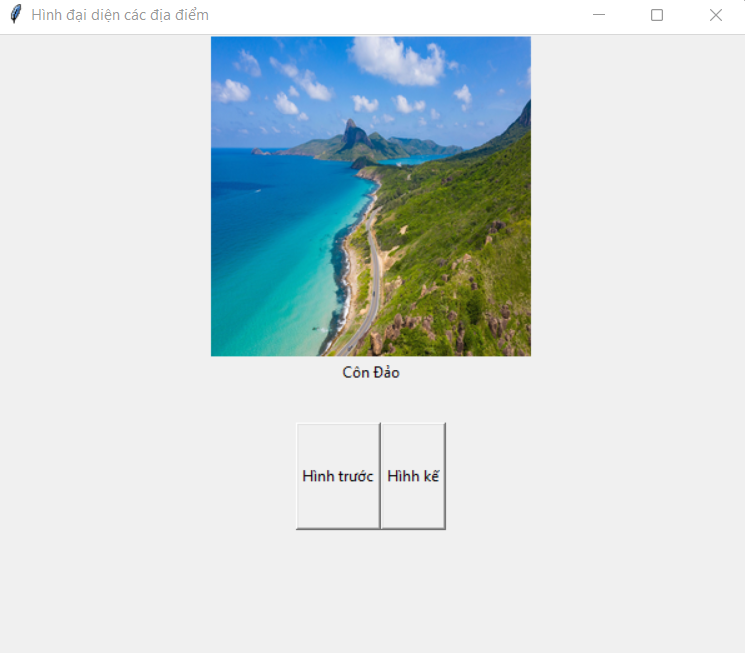
\includegraphics[scale=0.8]{instructions/down_all_avt_2}}
\caption{Tải tất cả hình ảnh đại diện}
\label{all2}
\end{figure}

\begin{figure}[H]
\center{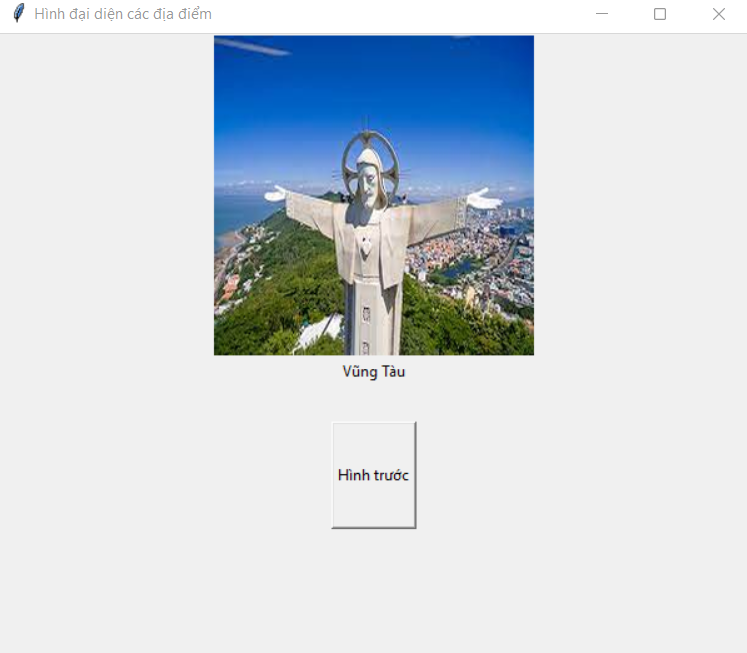
\includegraphics[scale=0.8]{instructions/down_all_avt_3}}
\caption{Tải tất cả hình ảnh đại diện}
\label{all3}
\end{figure}

\subsection{Tải các hình ảnh của một địa điểm}
Nút \textbf{Tải về hình ảnh} bên cạnh mỗi địa điểm cho phép client tải về tất cả hình ảnh của một địa điểm từ server. Hình ảnh sau khi tải về được xử lý tương tự như phần \ref{down_all_avt}. Các nút trong giao diện hiển thị hình ảnh cũng tương tự. Hình \ref{img1}, \ref{img2} và \ref{img3} là ví dụ về tải về các hình ảnh của một địa điểm.
\begin{figure}[H]
\center{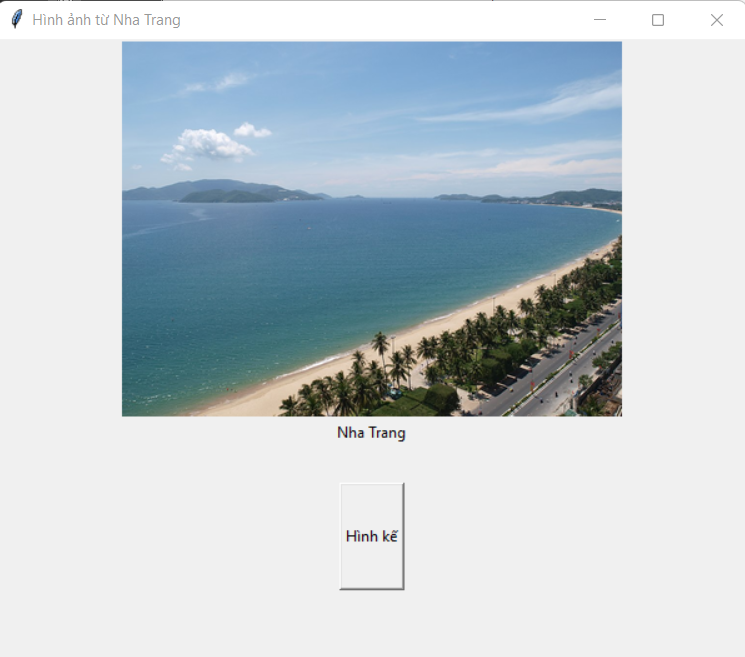
\includegraphics[scale=0.8]{instructions/down_all_img_1}}
\caption{Tải các hình ảnh của một địa điểm}
\label{img1}
\end{figure}

\begin{figure}[H]
\center{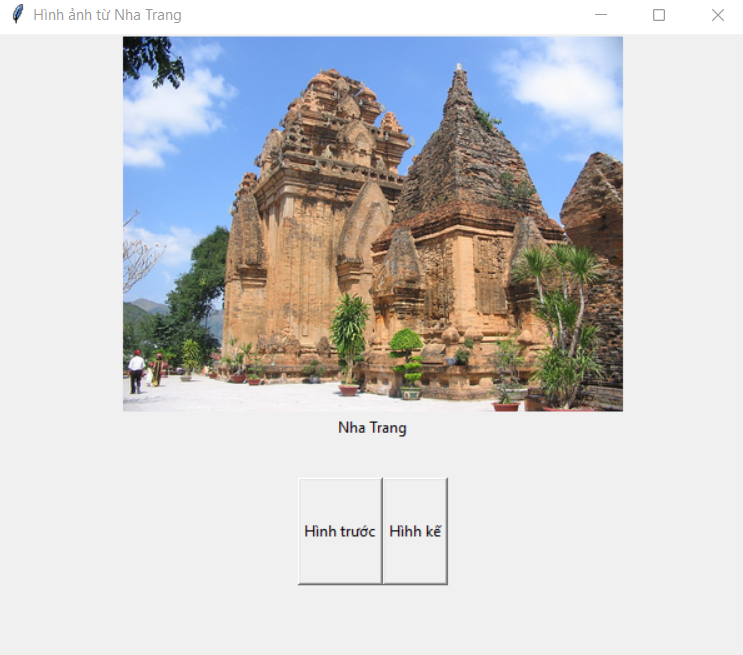
\includegraphics[scale=0.8]{instructions/down_all_img_2}}
\caption{Tải các hình ảnh của một địa điểm}
\label{img2}
\end{figure}

\begin{figure}[H]
\center{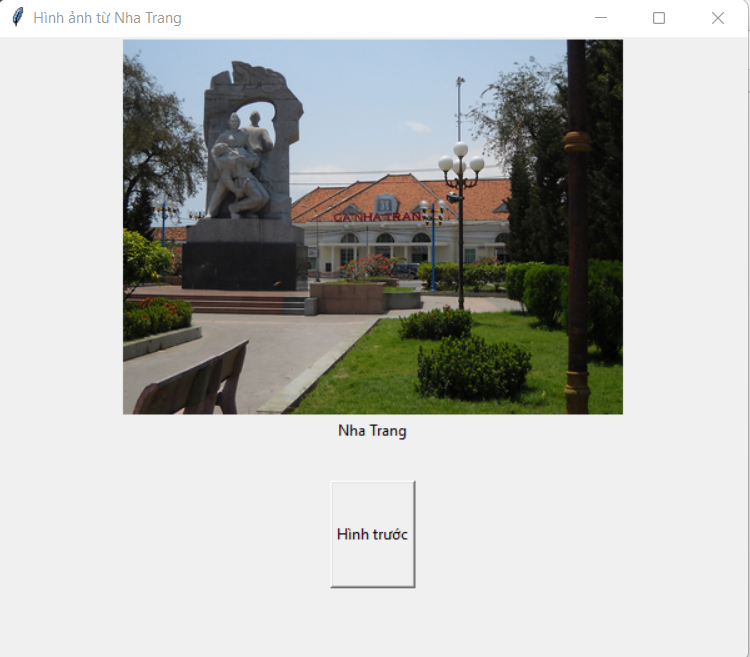
\includegraphics[scale=0.8]{instructions/down_all_img_3}}
\caption{Tải các hình ảnh của một địa điểm}
\label{img3}
\end{figure}

\subsection{Demo}
Demo của chương trình có thể được xem tại \href{https://youtu.be/K0q0q73HTxc}{đây}.\\
Link: \url{https://www.youtube.com/watch?v=K0q0q73HTxc}
